% !TeX root = ../proyecto.tex

\chapter{Implementación}\label{ch:implementacion}
En este capítulo se presenta en detalle la arquitectura técnica del sistema implementado, incluyendo los componentes y
módulos principales, las herramientas específicas empleadas en la construcción del sistema, y los elementos clave para
optimizar el rendimiento de los algoritmos y su evaluación.


\section{Descripción del Sistema}\label{sec:descripcion-del-sistema}
%Descripción del Sistema: Detalla la arquitectura del sistema que estás implementando.
La estructura del proyecto se organizó modularmente para facilitar el acceso, el mantenimiento y la extensibilidad del código fuente.
La organización de carpetas es la siguiente:
\begin{itemize}
      \item \texttt{data} -- Conjunto de datos utilizados en los experimentos.
      \item \texttt{docs} -- Documentación del proyecto en latex.
            \begin{itemize}
                  \item \texttt{bibliografia} -- Archivos relacionados con las referencias bibliográficas.
                  \item \texttt{capitulos} -- Archivos individuales para cada capítulo del documento.
                  \item \texttt{config} -- Archivos de configuraciones de la documentación LaTeX.
                  \item \texttt{imagenes} -- Imágenes utilizadas en la documentación.
                  \item \texttt{out} -- Archivos generados por el compilador de LaTeX.
                  \item \texttt{portada} -- Archivo portada del documento.
                  \item \texttt{prefacio} -- Archivo prefacio del documento.
                  \item \texttt{proyecto.tex} -- Archivo principal de LaTeX que compila el documento.
            \end{itemize}
      \item \texttt{img} -- Imágenes generadas automáticamente durante los experimentos.
      \item \texttt{LICENSE} -- Términos de distribución del proyecto.
      \item \texttt{logs} -- Registros de las ejecuciones, incluyendo tiempos de inicio, fin y resultados intermedios de los algoritmos.
      \item \texttt{README.md} -- Descripción general.
      \item \texttt{requirements.txt} -- Dependencias del proyecto.
      \item \texttt{results} -- Resultados de los experimentos.
            \begin{itemize}
                  \item \texttt{csvs} -- Resultados de las ejecuciones guardados en tablas.
                  \item \texttt{salidas} -- Salidas en bruto de consola.
            \end{itemize}
      \item \texttt{scripts} -- Scripts de ejecución automática, comparación de experimentos y generación de gráficos finales.
      \item \texttt{src} -- Código fuente principal del proyecto.
            \begin{itemize}
                  \item \texttt{algorithms} -- Implementaciones de los algoritmos.
                  \item \texttt{main.py} -- Módulo principal de ejecución individual.
            \end{itemize}
      \item \texttt{tmp} -- Ficheros temporales generados durante la ejecución.
      \item \texttt{utils} -- Módulos de apoyo, como clases auxiliares, generación de gráficos y funciones utilitarias.
\end{itemize}

El código completo del proyecto, incluyendo los scripts, algoritmos, documentación y resultados,
se encuentra disponible en el repositorio público de GitHub: \url{https://github.com/JoseRuizLopez/TFG}.


\section{Herramientas y Lenguajes de Programación}\label{sec:herramientas-y-lenguajes-de-programacion}
%Herramientas y Lenguajes de Programación: Lista las herramientas y tecnologías que usarás.
El desarrollo del proyecto se ha llevado a cabo utilizando \textbf{Python 3.10}~\cite{vanderplasPythonDataScience2016} como
lenguaje principal, debido a su versatilidad y amplia adopción en el campo del \textbf{aprendizaje profundo} y la
\textbf{manipulación de datos}.
Python es conocido por su facilidad de uso, extensibilidad y la gran cantidad de librerías disponibles para el
procesamiento de datos y la implementación de modelos de \textbf{machine learning}.


Las principales librerías empleadas durante el desarrollo son las siguientes:
\begin{itemize}
      \item \textbf{PyTorch 2.3.1}~\cite{ketkarIntroductionPyTorch2021, TorchcudaPyTorch24}: Para la construcción,
            entrenamiento y optimización de modelos de aprendizaje profundo.
            PyTorch fue elegido por su flexibilidad y capacidad para ejecutarse eficientemente en GPU\@.
      \item \textbf{Scikit-learn 1.5.2}~\cite{vanderplasPythonDataScience2016}: Para la evaluación de los modelos se utilizaron
            métricas estándar~\cite{kramerScikitLearn2016}.
            Su API permite una integración fluida con PyTorch y otros módulos.
      \item \textbf{Numpy 2.0.0}~\cite{NumPyV20Manual}: Para operaciones matemáticas y manipulación de matrices,
            siendo una herramienta esencial en el procesamiento de datos.
      \item \textbf{Polars 1.9.0}~\cite{PolarsPythonAPI}: Librería para manejar DataFrames de gran tamaño,
            elegida por su rendimiento superior en comparación con Pandas.
      \item \textbf{Pandas 2.2.3}~\cite{Pandas223Documentation}: Librería utilizada como apoyo para la generación de los gráficos,
            debido a las incompatibilidades detectadas con \texttt{polars}.
      \item \textbf{Matplotlib 3.9.2}~\cite{Matplotlib393Documentation}: Librería utilizada para la generación y
            visualización de gráficas.
      \item \textbf{Seaborn 0.13.2}~\cite{Seaborn0132Documentation}: Librería para la generación avanzada de gráficos estadísticos.
      \item \textbf{Openpyxl 3.1.5}~\cite{Openpyxl313Documentation}: Librería para la generación automática de archivos Excel a partir de resultados experimentales.
\end{itemize}

Cada una de estas herramientas fue seleccionada por su robustez y su idoneidad para cumplir con los requisitos
específicos del proyecto, facilitando tanto la implementación de los algoritmos meméticos como la reducción y el
análisis de los datos utilizados en los modelos de aprendizaje profundo.


\section{Gestión de Dependencias}\label{sec:gestion-de-dependencias}
Para garantizar que el proyecto se ejecute correctamente y todas las librerías necesarias estén disponibles,
se ha utilizado un archivo \texttt{requirements.txt}.
Este archivo contiene una lista de todas las librerías y sus versiones específicas que el proyecto requiere.

Para el \textbf{desarrollo local}, se ha optado por crear un entorno virtual utilizando
\texttt{venv}~\cite{CreationVirtualEnvironments}.
Esta práctica permite aislar las dependencias del proyecto de otros proyectos en la máquina, evitando conflictos entre
versiones de librerías.

Para la \textbf{implementación en el servidor}, se ha utilizado \texttt{conda}~\cite{CondaDocumentation} como gestor
de paquetes y entornos.
Conda facilita la gestión de entornos y la instalación de librerías, especialmente en configuraciones más complejas.

Esto facilita la reproducibilidad del proyecto y minimiza posibles conflictos de versión, lo que es fundamental para
mantener la integridad del código y el rendimiento de las aplicaciones.


\section{Arquitectura de la Implementación}\label{sec:arquitectura-de-la-implementacion}
La arquitectura de la implementación desarrollada para este trabajo está diseñada con un enfoque modular y escalable,
que permite gestionar de forma eficiente las distintas fases del proceso de selección de instancias y evaluación de modelos.
El sistema se compone de varios módulos interrelacionados que se encargan de la generación de subconjuntos,
la ejecución de los algoritmos evolutivos y meméticos, la evaluación de las soluciones mediante modelos preentrenados, y la visualización y almacenamiento de resultados.
Esta estructura facilita la incorporación de nuevos algoritmos o mejoras en los ya existentes, garantizando una mayor flexibilidad y mantenimiento del código.

\subsection{Esquema General de Funcionamiento de los Algoritmos}\label{subsec:esquema-algoritmos}
El funcionamiento general de los algoritmos implementados en este trabajo sigue un flujo estructurado y modular que permite una ejecución ordenada de todas las etapas del proceso.
La Figura~\ref{fig:esquema-flujo-algoritmos} muestra el esquema general de funcionamiento, desde la configuración inicial hasta la evaluación final de resultados.

\begin{figure}[htp]
      \centering
      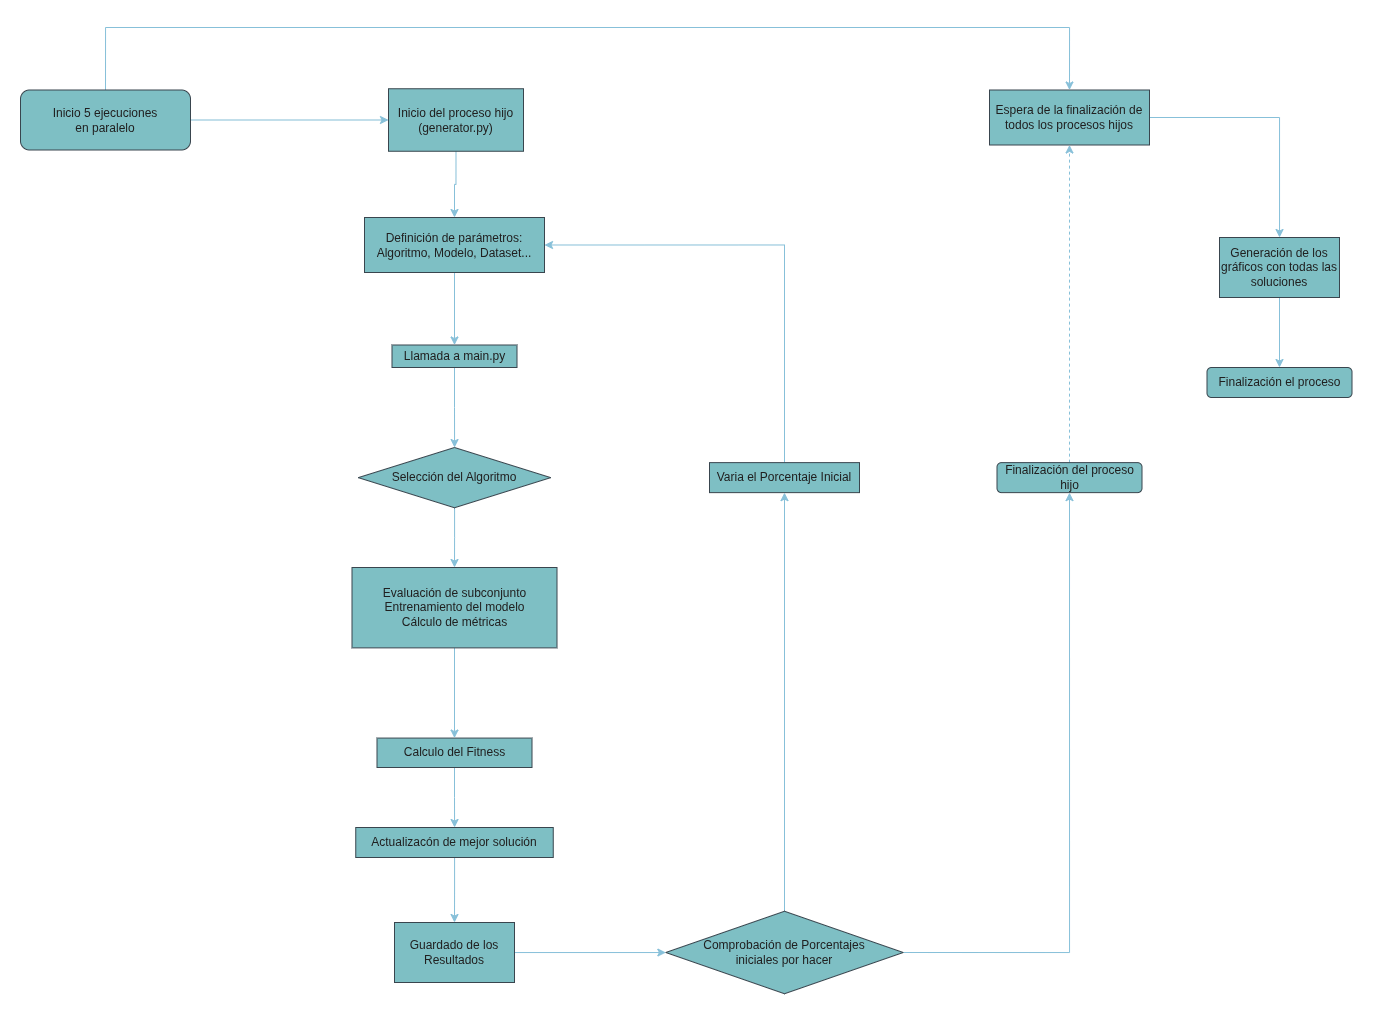
\includegraphics[width=0.95\textwidth]{imagenes/flujo2.drawio}
      \caption{Esquema general del flujo de ejecución de los algoritmos y evaluación de subconjuntos.}
      \label{fig:esquema-flujo-algoritmos}
\end{figure}

El proceso se organiza en los siguientes pasos principales:

\begin{enumerate}
      \item \textbf{Ejecución del script de paralelización:} Se inicia el script que permite ejecutar múltiples experimentos de manera paralela,
            facilitando la obteción de resultados de diferentes semillas.
      \item \textbf{Configuración inicial:} Se define el algoritmo, el modelo y el dataset a utilizar, a través de los parámetros en \texttt{generator.py}.
      \item \textbf{Ejecución del núcleo principal:} El script \texttt{main.py} se encarga de orquestar la ejecución,
            llamando a las funciones específicas según el algoritmo seleccionado.
      \item \textbf{Generación y evaluación de subconjuntos:} Cada algoritmo genera subconjuntos de datos de entrenamiento a partir del conjunto original.
      \item \textbf{Entrenamiento del modelo:} Se realiza el entrenamiento del modelo utilizando los subconjuntos generados,
            aplicando técnicas de \textit{transfer learning} con modelos preentrenados.
      \item \textbf{Almacenamiento de resultados:} Cada evaluación almacena los resultados obtenidos (métricas y composición del subconjunto) y,
            tras finalizar la ejecución, se generan gráficos como boxplots y visualizaciones que permiten analizar el rendimiento de cada enfoque.
\end{enumerate}

\subsection{Configuración de Modelos Preentrenados}\label{subsec:configuracion-modelos-preentrenados}
En este trabajo, se han utilizado modelos convolucionales preentrenados como base para la tarea de clasificación de imágenes.
Concretamente, se han empleado las arquitecturas \textbf{ResNet50} y \textbf{MobileNetV2},
cargadas con pesos preentrenados sobre \texttt{ImageNet} o \texttt{CIFAR10}, según el dataset utilizado en cada experimento.

Para adaptar estos modelos a la tarea específica de clasificación de subconjuntos de datos,
se ha seguido una estrategia de \textit{transfer learning} que permite reducir significativamente el coste computacional del entrenamiento.
Esta estrategia consiste en congelar todas las capas del modelo, excepto la última,
de manera que las representaciones aprendidas en la etapa preentrenada puedan ser reutilizadas como extractores de características generales.

Específicamente, la \textbf{última capa} de cada modelo preentrenado (la capa densa o \textit{fully connected})
ha sido reemplazada por una nueva capa completamente conectada (\texttt{Linear}) adaptada al número de clases del dataset en uso.
Esta capa es la única que se entrena durante la fase de evaluación de cada subconjunto generado por los algoritmos,
permitiendo obtener métricas como \textit{accuracy}, \textit{precision}, \textit{recall} y \textit{F1-score} de forma eficiente.

El uso de pesos preentrenados y la congelación de capas proporcionan varias ventajas:
\begin{itemize}
      \item Reducción del tiempo de entrenamiento en cada evaluación.
      \item Aprovechamiento de representaciones genéricas previamente aprendidas, lo que mejora la generalización.
      \item Adaptabilidad de los modelos a distintos datasets y tareas, modificando únicamente la capa final.
\end{itemize}

Este enfoque se implementa mediante las herramientas de PyTorch,
congelando explícitamente los gradientes de todas las capas del modelo y definiendo la nueva capa final con el número adecuado de salidas para cada problema de clasificación.

\subsection{Módulo de Algoritmos}\label{subsec:modulo-de-algoritmos}
Ubicado en \texttt{src/algorithms/} este módulo contiene las implementaciones principales de los
algoritmos desarrollados en el proyecto.

Este módulo utiliza la arquitectura GPU para maximizar la velocidad de ejecución y está diseñado para ser escalable,
permitiendo la inclusión de nuevos operadores meméticos si es necesario.

\subsection{Núcleo de Ejecución}\label{subsec:nucleo-de-ejecucion}
El módulo \texttt{main.py} centraliza la ejecución de un experimento individual, inicializando configuraciones,
entrenando el modelo y generando gráficos.

Los pasos de la función principal de \texttt{main.py} es:
\begin{enumerate}
      \item \textbf{Establece Configuración Inicial}: Configura una semilla, elige el dataset y prepara un archivo de log.
      \item \textbf{Inicia el Proceso del Algoritmo}: Según el nombre del algoritmo (algoritmo) especificado, se llama a
            la función correspondiente (por ejemplo, genetic\_algorithm, memetic\_algorithm, etc.).
      \item \textbf{Almacena Resultados}: Una vez que el algoritmo termina, registra la duración, los resultados y la
            métrica final en un archivo.
      \item \textbf{Visualiza Resultados}: Si hay datos de fitness, genera una gráfica de la evolución del fitness a lo
            largo del proceso.
      \item \textbf{Genera un Resumen}: Calcula estadísticas adicionales (como porcentaje de clases seleccionadas en
            Paper, Rock y Scissors), y devuelve estos resultados junto con el historial de fitness.
\end{enumerate}

\subsection{Módulo de Utilidades}\label{subsec:modulo-de-utilidades}
La carpeta \texttt{utils/} contiene funciones auxiliares:
\begin{itemize}
      \item \textbf{utils\_plot.py}: Generación de gráficos.
      \item \textbf{classes.py}: Definición de enumeraciones para algoritmos, métricas, datasets y modelos.
      \item \textbf{utils.py}: Funciones de ayuda como el cálculo de métricas o la creación de diccionarios de selección de imágenes.
\end{itemize}

Estos módulos se encargan de generar gráficas comparativas entre distintos porcentajes o algoritmos y en
generar un CSV con los datos finales para ser analizados.

\subsection{Scripts de Ejecución en GPU}\label{subsec:scripts-de-ejecucion-en-gpu}
En scripts, se encuentran los programas necesarios para ejecutar los algoritmos en un servidor GPU, lo que permite
maximizar la eficiencia en el entrenamiento y la evaluación de modelos.
\begin{enumerate}
      \item \textbf{Configuración de GPU}: Los scripts están configurados para identificar y utilizar las GPU disponibles
            en el servidor, reduciendo los tiempos de entrenamiento de modelos.
      \item \textbf{Optimización de Ejecución}: Se implementaron configuraciones de batch size y técnicas de
            procesamiento paralelo en PyTorch, aprovechando la memoria y el poder de procesamiento de las GPU\@.
\end{enumerate}

Estos scripts están diseñados para ser ejecutados en un entorno de servidor, reduciendo los tiempos de prueba en el
entorno local y permitiendo un análisis iterativo más rápido.


\section{Consideraciones de Optimización}\label{sec:consideraciones-de-optimizacion}
Durante el desarrollo, se optimizaron varios aspectos para mejorar el rendimiento del sistema:

\begin{enumerate}
      \item \textbf{Aceleración en GPU}: Todas las operaciones de cálculo intensivo fueron migradas a la GPU mediante
            PyTorch.
      \item \textbf{Uso Eficiente de Memoria}: Con Polars y Numpy, se optimizó el manejo de grandes volúmenes de datos,
            utilizando tipos de datos específicos para reducir el uso de memoria.
      \item \textbf{Automatización de Evaluaciones}: Las pruebas de rendimiento se automatizaron, permitiendo una
            evaluación continua sin intervención manual.
      \item \textbf{Control de reproducibilidad}: Se fijaron semillas aleatorias en todas las librerías involucradas
            (random, numpy, torch, cuda) y se desactivaron los algoritmos no deterministas de cuDNN~\cite{CuBLASDeterministicAlgorithms}.
            Esta medida garantiza que las ejecuciones del sistema produzcan resultados consistentes entre sesiones,
            algo esencial en entornos de evaluación comparativa.
      \item \textbf{Diagnóstico automático de GPU}: Implementación de un script (cuda-diagnostic.py) que comprueba disponibilidad
            de CUDA y dispositivos antes de lanzar experimentos, garantizando un entorno correcto.
\end{enumerate}

Además, se implementó un mecanismo de \textbf{early stopping} basado en la ausencia de mejora del valor de fitness durante
un número determinado de evaluaciones consecutivas.
Aunque no se utiliza una pérdida de validación explícita como en enfoques tradicionales, este enfoque funcionalmente cumple el mismo propósito:
detener el algoritmo cuando se detecta estancamiento, reduciendo así el coste computacional innecesario~\cite{EarlyStoppingDiscussion2024}.

Gracias a estas optimizaciones, el sistema permite explorar un amplio abanico de configuraciones de manera eficiente, manteniendo la robustez y estabilidad de los resultados.


\section{Métricas de Evaluación}\label{sec:metricas-evaluacion}
Para evaluar el rendimiento de los modelos de clasificación utilizados en los experimentos,
se han empleado cuatro métricas estándar en el ámbito del aprendizaje automático: \textbf{accuracy}, \textbf{precisión}, \textbf{recall} y \textbf{F1-score}.
Dado que se trata de un problema multiclase, estas métricas se han calculado utilizando el promedio \textit{macro},
lo que implica computarlas individualmente para cada clase y luego obtener la media aritmética.

A continuación se describen y formalizan cada una de estas métricas:

\begin{itemize}
      \item \textbf{Accuracy} (exactitud): representa la proporción de predicciones correctas sobre el total de ejemplos.
            $$
                  Accuracy = \frac{TP + TN}{TP + TN + FP + FN}
            $$
            En el caso multiclase, se generaliza como:
            $$
                  \mathrm{Accuracy} = \frac{\text{Número de predicciones correctas}}{\text{Total de predicciones}}
            $$

      \item \textbf{Precisión}: mide cuántas de las instancias clasificadas como positivas fueron realmente positivas.
            En el caso multiclase (macro), se calcula como:
            $$
                  \text{Precisión}_{\text{macro}} = \frac{1}{C} \sum_{i=1}^{C} \frac{TP_i}{TP_i + FP_i}
            $$

      \item \textbf{Recall}: indica cuántas de las instancias realmente positivas fueron correctamente identificadas por el modelo:
            $$
                  \mathrm{Recall}_{\text{macro}} = \frac{1}{C} \sum_{i=1}^{C} \frac{TP_i}{TP_i + FN_i}
            $$

      \item \textbf{F1-score}: es la media armónica entre precisión y recall, útil cuando se desea un equilibrio entre ambas:
            $$
                  \mathrm{F1\text{-}score}_{\text{macro}} = \frac{1}{C} \sum_{i=1}^{C} \frac{2 \cdot \text{Precisión}_i \cdot \text{Recall}_i}{\text{Precisión}_i + \text{Recall}_i}
            $$
\end{itemize}

Donde:
\begin{itemize}
      \item $TP_i$: verdaderos positivos de la clase $i$
      \item $FP_i$: falsos positivos de la clase $i$
      \item $FN_i$: falsos negativos de la clase $i$
      \item $C$: número total de clases
\end{itemize}

Para facilitar la comprensión de estos conceptos, en la Figura~\ref{fig:matriz-confusion} se muestra una representación gráfica de una matriz de confusión.
\begin{figure}[H]
      \centering
      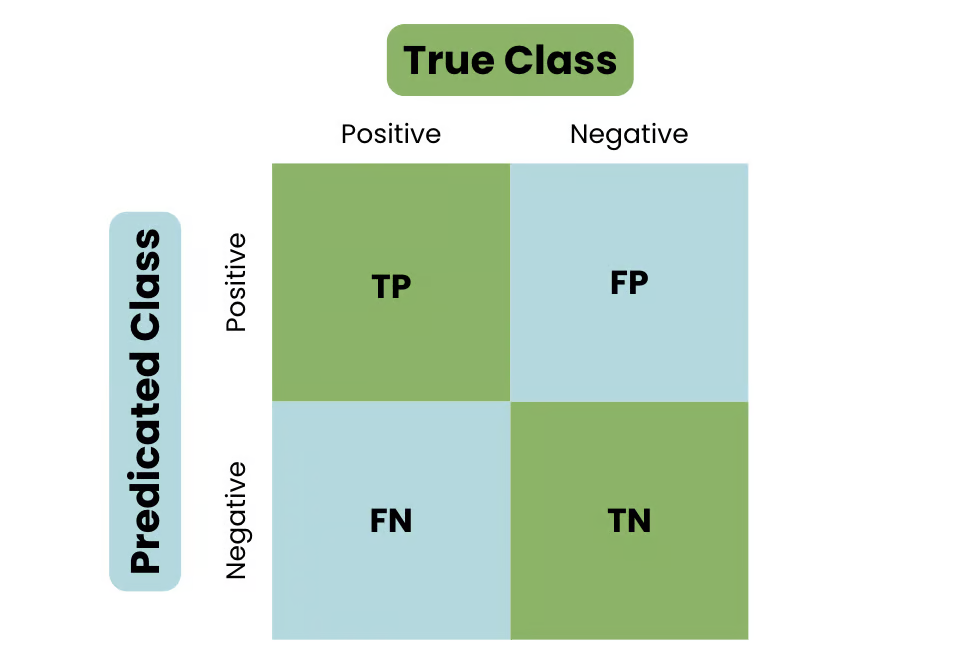
\includegraphics[width=0.5\textwidth]{imagenes/matriz-de-confusion.png}
      \caption{Representación gráfica de una matriz de confusión}
      \label{fig:matriz-confusion}
\end{figure}

Estas métricas fueron implementadas utilizando la librería \texttt{scikit-learn}, que permite su cálculo eficiente a partir de las
predicciones del modelo y las etiquetas reales del conjunto de validación.
